\documentclass[spanish, fleqn]{scrartcl}
\usepackage[utf8]{inputenc}
\usepackage[english]{babel}
\usepackage[paper=a4paper, top=2cm, left=2cm, right=2cm]{geometry}
\usepackage{tikz}
\usepackage{CIACcustom}
\usepackage{amsmath, amsthm}
\usepackage{listings}
\usepackage{multicol}
\usepackage{fancyhdr}
\usepackage[urlcolor=blue, colorlinks]{hyperref}
\usepackage{booktabs,tabularx}
\usepackage{float}


\newcolumntype{L}[1]{>{\hsize=#1\hsize\raggedright\arraybackslash}X}%
\newcolumntype{R}[1]{>{\hsize=#1\hsize\raggedleft\arraybackslash}X}%
\newcolumntype{C}[2]{>{\hsize=#1\hsize\columncolor{#2}\centering\arraybackslash}X}%

\pagestyle{fancy}
\fancyhf{}
\rhead{\pgfimage[width=2.5cm]{imagenes/logo-ciac.png}}
\chead{
  Apoyos intensivos Guía Nro 3 Parte 1\\
  IWI-131 Semestre II-2016 \\
  CIAC Casa Central
}
\lhead{\pgfimage[width=2.5cm]{imagenes/logo-usm.jpg}}
\rfoot{\LaTeXe / CIAC 2016}
\lfoot{\thepage}

\renewcommand{\ttdefault}{pcr}

%%% listings settings:
\definecolor{bggray}{rgb}{0.95,0.95,0.95}
\lstdefinestyle{consola}{
  backgroundcolor=\color{bggray},
  basicstyle=\small\ttfamily,
  frame=single,
  moredelim=[is][\bfseries]{[*}{*]},
  xrightmargin=5pt
}

\lstdefinestyle{mypy}{
  language=python,
  backgroundcolor=\color{bggray},
  basicstyle=\ttfamily\small\color{orange!70!black},
  frame=L,
  keywordstyle=\bfseries\color{green!40!black},
  commentstyle=\itshape\color{purple!40!black},
  identifierstyle=\color{blue},
  stringstyle=\color{red},
  numbers=left,
  showstringspaces=false,
  xrightmargin=5pt,
  xleftmargin=10pt
}

\newtheorem{CIACdef}{Definición}

\begin{document}
% \vspace*{.3cm}
% \section{Contabilidad Básica}

Un antiguo ingeniero comercial que olvidó como programar le pide ayuda a usted en el balance de cuentas de su empresa. Algunas cuentas se corrigen monetariamente en base al IPC y otras se deprecian.

Se tienen dos archivos \texttt{archivos.txt} y \texttt{pasivos.txt}. Dentro de ellos hay dos tipos de formas, \texttt{cuenta; indicacion; monto} y \texttt{cuenta; indicacion; valor\_residual; vida\_útil; monto}, esta última es para bienes que se deprecian.

\begin{figure}[h]
    \centering
    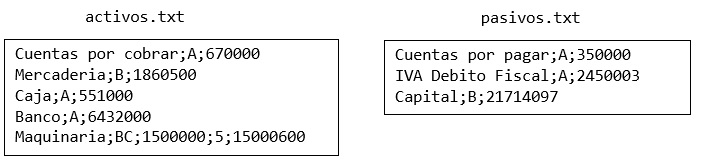
\includegraphics{Imagenes/imagen1.jpg}
\end{figure}

Las indicaciones son:
\begin{itemize}
    \item[A:] No existe ningún cambio
    \item[B:] Hay ajuste monetario por IPC
    \item[C:] Se deprecia
\end{itemize}

Afortunadamente para usted, este ingeniero aún no necesita depreciar sus bienes. 
Se tiene un diccionario \texttt{valores\_IPC} cuyas llaves son tuplas de fechas (año,mes) y sus valores son los puntos del IPC

\begin{lstlisting}[style=consola]
valores_IPC={
(2016,1):111.39, (2016,2):111.70, (2016,3):112.13,
(2016,4):112.49, (2016,5):112.75, (2015,1):106.30, (2015,2):106.68,
(2015,3):107.35, (2015,4):107.97, (2015,5):108.16, (2015,6):108.68,
(2015,7):109.14, (2015,8):109.88, (2015,9):110.44, (2015,10):110.89,
(2015,11):110.86, (2015,12):110.87}
\end{lstlisting}

Cree las funciones:
\begin{itemize}
    \item[a.] \texttt{total(archivo)} que recibiendo un string de un archivo retorne un entero con la suma total de los montos indicados en el archivo.
    \item[b.] \texttt{correccion(archivo,actual,inicial)} que reciba un string con el nombre del archivo a corregir y dos tuplas con el mes actual e inicial de forma (año,mes). Esta función debe actualizar el monto siguiendo las indicaciones dadas. Se entenderá que para corregir un monto se multiplicará por la razón de los valores del IPC de la fecha actual y la fecha inicial.
\end{itemize}

\paragraph{Aclaraciones} Lo del ingeniero comercial es mentira. La corrección monetaria se calcula de otra forma, pero para efectos de algoritmo se ha simplificado.
% \newpage
\section*{Resumen, Recetario, Formulario, Paltario, etc}

\subsection*{Tuplas}

\begin{itemize}
    \item Para inicializar una tupla use:
\begin{lstlisting}[style=consola]
tupla=(datos) #o bien
tupla=tuple(datos)
\end{lstlisting}
    \item Las tuplas no se pueden modificar una vez creadas, sólo reemplazándolas en la variable original. No tienen funciones propias (son inmutables).
    \item Se pueden desempaquetar, o asignar variables a sus elementos, por ejemplo
\begin{lstlisting}[style=consola]
>>>(nombre,apellido)=('Miguel','Godoy')
>>>nombre
'Miguel'
>>>apellido
'Godoy'
\end{lstlisting}
    \item Se pueden comparar
\begin{lstlisting}[style=consola]
>>>(1,2,3)>(1,2)
True
>>>(2,4,5)<(2,5,6)
True
>>>(1,2)==(2-1,10\%8)
True    
\end{lstlisting}
    \item Se pueden concatenar
\begin{lstlisting}[style=consola]
>>>(1,2,3)+(0,0,1)
(1,2,3,0,0,1)
\end{lstlisting}
\end{itemize}

\subsection*{Listas}

\begin{itemize}
    \item Se pueden comparar y concatenar de la misma forma que las tuplas
    \item Para inicializarlas
\begin{lstlisting}[style=consola]
lista=[] #o bien
lista=list()
\end{lstlisting}
    \item Para agregar elementos
\begin{lstlisting}[style=consola]
lista.append(dato) #o si lista ya esta creada
lista=lista+[dato]
\end{lstlisting}
 
    \item Para eliminar un dato de la lista
\begin{lstlisting}[style=consola]
lista.remove(elemento) #Conociendo el elemento a eliminar
del lista[indice] #Conociendo el indice del elemento a eliminar
\end{lstlisting}

    \item Algunos comandos varios son 
\begin{lstlisting}[style=consola]
lista.sort() #Ordena de menor a mayor la lista, RETORNA NONE
lista.reverse() #Invierte el orden de los elementos RETORNA NONE
\end{lstlisting}

    \item Tener cuidado con la asignación de una variable para una misma lista

\begin{lstlisting}[style=consola]
>>> lis_a=[1,3,2]
>>> lis_b=lis_a
>>> lis_b.remove(3)
>>> lis_a
[1, 2]
>>> lis_b
[1, 2]
\end{lstlisting}
Lo anterior pasa porque se asignan dos variables al mismo espacio de memoria, para evitar esto se hace
\begin{lstlisting}[style=consola]
>>> lis_a=[1,3,2]
>>> lis_b=list(lis_a) #Se asegura que sea una lista nueva
>>> lis_b.remove(3)
>>> lis_a
[1, 3, 2]
>>> lis_b
[1, 2]
\end{lstlisting}

\end{itemize}

\subsection*{Ciclo for}

Anteriormente para recorrer una estructura de tipo string, nos aprovechábamos de que podemos acceder a cada caracter usando un índice de la forma:

\begin{lstlisting}[style=consola]
cadena='Programacion'
contador=0
while contador<len(cadena):
    print(cadena[contador], end="")
    contador+=1
\end{lstlisting}

Que imprime
\begin{lstlisting}[style=consola]
P r o g r a m a c i o n
\end{lstlisting}

Lo anterior se puede seguir usando, pero existe una forma más compacta de recorrer estructuras usando el comando \texttt{for}

\begin{lstlisting}[style=consola]
cadena='Programacion'
for caracter in cadena:
    print(caracter, end="")
\end{lstlisting}

Que imprime lo mismo.

Para recorrer una estructura de listas con tuplas que deben desempaquetarse, como por ejemplo
\begin{lstlisting}[style=consola]
capitales=[('Chile','Santiago'),('Argentina','Bs. Aires'),('Alemania','Berlin')]
\end{lstlisting}
Se puede
\begin{itemize}
    \item[1.] Desempaquetar inmediatamente 
    \begin{lstlisting}[style=consola]
for pais,capital in capitales:
    print('La capital de', pais, 'es', capital)
    \end{lstlisting}
    
    \item[2.] Desempaquetar en un paso siguiente
    \begin{lstlisting}[style=consola]
for tupla in capitales:
    pais,capital=tupla
    print('La capital de',pais,'es',capital)
    \end{lstlisting}
    
    \item[3.] No desempaquetar, y usar índices para referirse a los datos
    \begin{lstlisting}[style=consola]
for tupla in capitales:
    print('La capital de',tupla[0],'es',tupla[1])
    \end{lstlisting}
\end{itemize}
\end{document}